\chapter{Next Steps und Zukunftsperspektiven}
\section{Einführung}
Im laufe der Geschichte sorgten viele Ereignisse, wie Kriege, Naturkatastrophen und andere Geschehnisse globalen Ausmaßes dafür, dass sich das Verhalten der Menschen nachhaltig änderte.
Durch die Covid-19 Pandemie ist die Digitalisierung weltweit weiter in den Fokus gerückt als je zuvor.
Akteure in Wirtschaft, Politik und Wissenschaft werden gezwungen eigene Digitalisierungsmaßnahmen stark zu beschleunigen.
Digitalisierung ist nun nicht mehr nur der neue Trend des Jahrhunderts, sondern das notwendige Übel, ohne welches die Welt zum Stillstand kommt.

Auch auf die Planung und Ausführung von Konferenzen lässt sich dieser Trend übertragen.
Zwar ist davon auszugehen, dass bis zum Jahr 2022 pyhsische Veranstaltungen wenigstens im eingeschränkten Rahmen wieder möglich sind, so ist es auch zu erwarten, dass viele Menschen digitalen Zugang zu Veranstaltungen und deren Ressourcen fordern.
Daher ist es zwingend notwending, dass als weitere Schritte der Konferenzplanung digitale Aspekte noch stärker berücksichtigt werden müssen.

Weiterhin zeigt der Trend des letzten Jahrzenhts eine Entwicklung hin zur Nutzung mobiler Anwendung und einer immer stärkeren Marktpenetration mobiler Endgeräte.
Allein in Deutschland besitzen 89\% aller Menschen ein Smartphone.
Sogar in der Generation 65+ liegt der Anteil 2020 bei etwa 79\%.
Von den Deutschen Smartphonenutzern verwenden beinahe 95\% ihr Gerät täglich, etwa um Nachrichten zu verschicken, oder Social Media Kanäle zu pfelgen und zu verfolgen. \autocite[]{B_Gentner.2020}

% Partnerschaften mit Hotels für Zimmer
% Auswahl der Paper
\section{App Konzept für die \ac{MOBTS} Konferenz}
Aus dem dargelegten Trend kann eine gewisse Notwendigkeit für mobile Anwendungen für Konferenzen hergeleitet werden.
Da sich die Nutzung mobiler Anwendungen einer nie dagewesenen Beliebtheit erfreut, muss eine mobile Applikation (App) als vielversprechende Methode verstanden werden, mehr Aufmerksamkeit auf die \ac{MOBTS} Konferenzen zu lenken.
Zum einen kann eine mobile App den Zugang zur Konferenz selbst vereinfachen, sie kann aber auch für eine bessere Erfahrung der Konferenzbesucher sorgen, indem sie einfachen Zugang zu Ressourcen schafft.
Im Folgenden sollen daher die Anforderungen an eine solche App analysiert und dargelegt werden und ein ersten Konzept erarbeitet werden, sowie Vorschläge zu zu verwendenden Technologien gemacht werden.

Dazu wird zunächst untersucht, wie die gegenwärtige Erfahrung eines Besuchers auf einer \ac{MOBTS} Konferenz aussieht und an welchen Stellen eine App Verbesserungen schaffen kann.
Nach und nach soll hier aus eine zuerst relativ abstrakten Vision ein konkretes Konzept erarbeitet werden.

\subsection{Problembeschreibung}
Ein Besucher der \ac{MOBTS} Konferenz fordert ein Ticket an, welches zum Besuch der Konferenz berechtigt.
Besagten Ticket erreicht den Besucher nun vermutlich per Email oder postalisch.
Wird das Ticket per Email verschickt, ist die Wahrscheinlichkeit hoch, dass es sogleich ausgedruckt wird.
In jeden Fall ist das Resultat also ein Stück Papier, welches zum Besuch der Konferenz mitgenommen wird.
Am Ort der Konferenz wird besagtes Stück Papier am Empfangstisch oder einer ähnlichen Einrichtung gegen eine Plakette oder einen Ausweis eingetauscht, welchen der Besucher während des gesamten Verlaufs der Konferenz mit sich herumträgt.

Über den Ablauf der Konferenz hat sich der Besucher vermutlich bereits im Voraus informiert, allerdings ist es auch denkbar, dass am Konferenzort Ablauf- und Raumpläne konsultiert werden. 
Gerade letztere werden zur Orientierung genutzt und sind entweder an versschiedenen Stellen im Konferenzgeäude zu finden oder als abgespeichertes PDF, Screenshot oder wieder in ausgedruckter Form selbst von den Besuchern mitgebracht.
Nachteilig hierbei ist, dass die ausgehängten Pläne schwer zu finden sein können und die eigens mitgebrachten eventuelle Planänderungen nicht enthalten.
Die Informationsfindung kann sich also unter Umständen schwierig gestalten.

Für das Besuchen der einzelnen Sessions und Vorträge sind auch einige Verhaltensmuster der Besucher festzustellen.
So werden beispielsweise Vorlagen für die Aufzeichnung von Notitzen vom Veranstalter bereitgestellt, die von den Besuchern genutzt werden.
Eine solche vereinfachte Vorlage wird in \autoref{fig:notes-template} dargestellt.
Auch hier wird die Vorlage in den Tagen vor der Konferenz mehrfach ausgedruckt und in Papierform mitgenommen.

\begin{figure}
    \begin{center}
        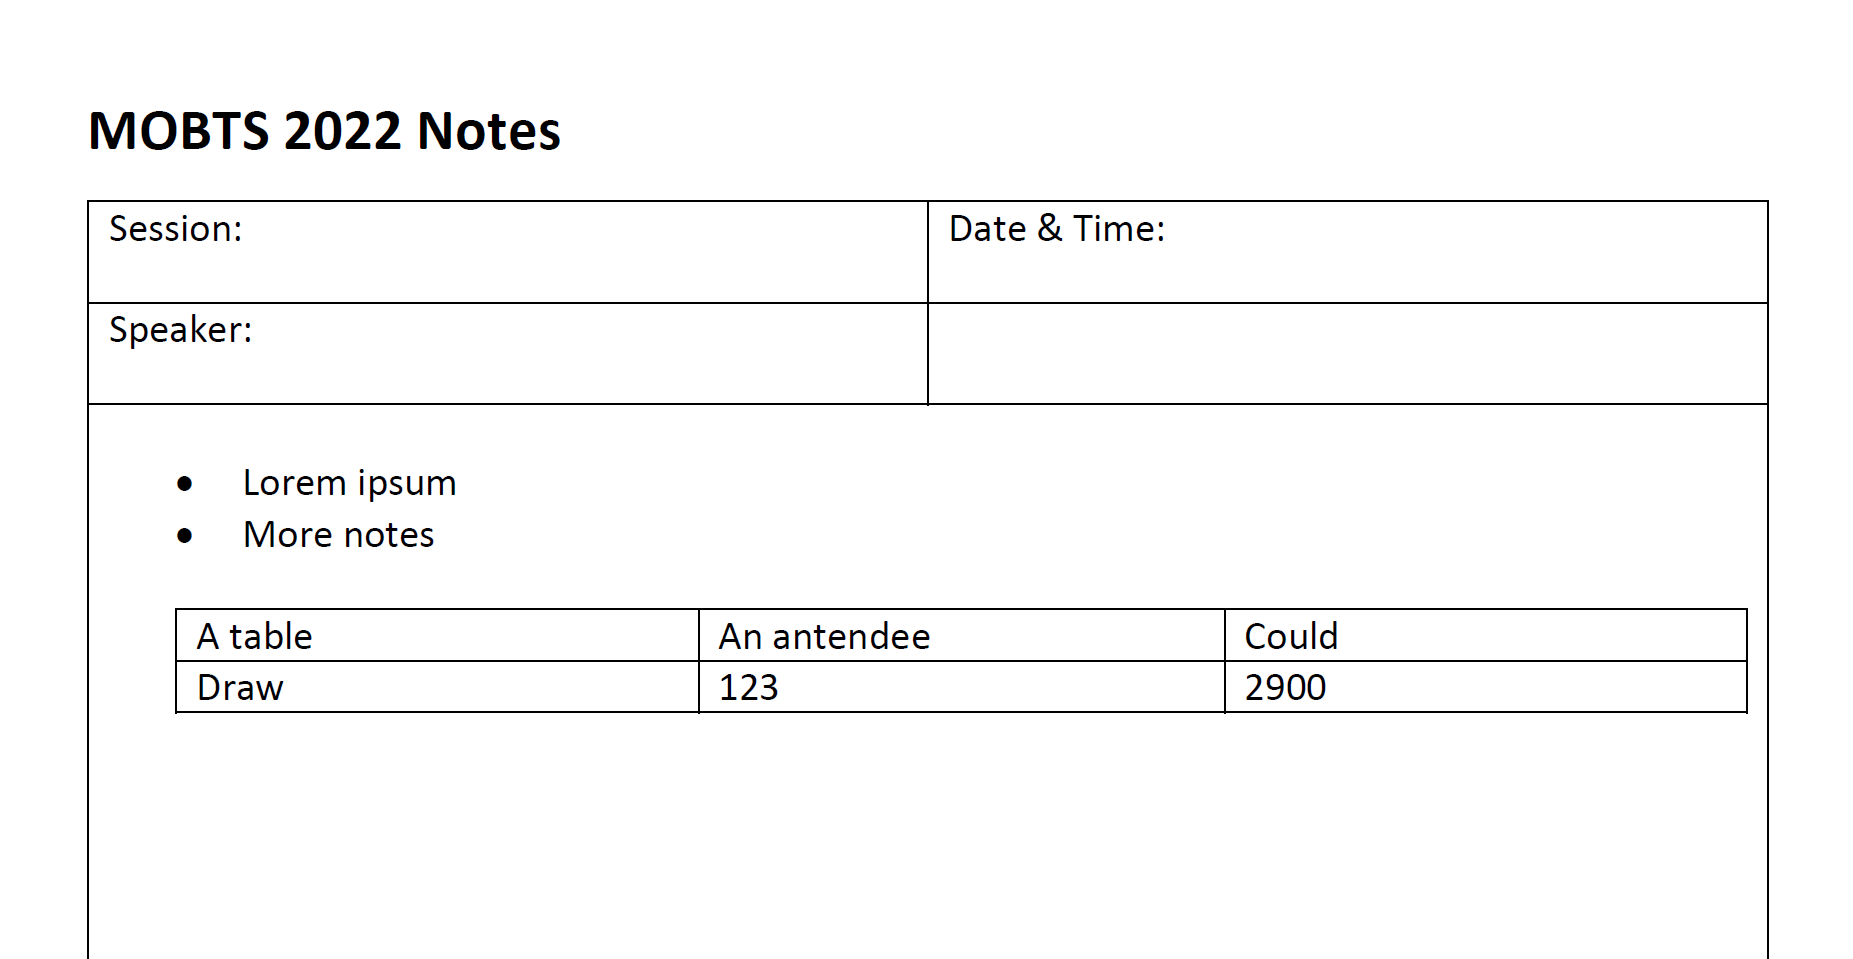
\includegraphics[width=0.9\textwidth]{img/notes_template.PNG}
    
    \end{center}
    \caption{Vereinfache Notizen Vorlage}
    \label{fig:notes-template}
\end{figure}

Da aufgrund der gegenwärtigen Situation ein Teil der Konferenz digital stattfinden wird, ist davon auszugehen, dass Vorträge uns andere Sessions wenigstens zu einem gewissen Grad auch aufgezeichnet werden.
Wie oder wo diese Aufzeichnungen zugänglich sein werden, ist allerdings unklar, womit auch das (digitale) Auffinden von Ressourcen nicht klar organisiert zu sein scheint. 

\subsection{Anforderungen}
Aus der dargelegten Problembeschreibung soll zunächst eine high-level Vision für eine mögliche App abgeleitet werden.
Als grundlegendes Problem kann hier eine fehlende Digitalisierung der Konferenzressourcen und eine fehlende Zentralisiertung identifiziert werden.
Wichtige Dokumente werden ausgedruckt verwendet und Informationen sind nicht einfach zentral an einem Ort abrufbar.
Die Idee einer App stellt sich also in der Beantwortung der Frage \enquote{Wo finde ich X?} mit \enquote{In der \ac{MOBTS} App.} dar.
Alle relevanten Informationen die vor, während und nach der Konferenz benötigt werden, sollen an einem einzigen Punkt einfach zugänglich gemacht werden.

\subsubsection*{Vor der Konferenz}
\textbf{Allgemeine Informationen} zu den \ac{MOBTS} Konferenzen, Neuigkeiten und sonstige Inhalte, die gegnwärtig auf der Website der \ac{MOBTS} \url{https://mobts.org/} angeboten werden, sollen in der App einsehbar sein.
So sollen sich Interessenten und mögliche Besucher einfach einen Überblick verschaffen können.

\textbf{Tickets} und Informationen zum Besuch der \ac{MOBTS} sollen auch in der App verfügbar sein.
Denkbar hier ist, dass bei Erwerb eines Ticket ein Nutzeraccount in der App angelegt wird, über den der Besucher sein Ticket speichern kann und auf weitere Informationen zur Konferenz zugreifen kann.
Die App kann das gespeichert Ticket bei Anmeldung am Konferenzort in Form eines QR-Codes oder durch \ac{NFC} nutzen, um den Besucher zu identifizieren und eine Badge auszustellen.
So entfällt die Notwendigkeit ein Ticket ausdrucken und mitbringen zu müssen.
Außerdem ist so gesichert, dass die Tickets zentral auf der Infrastruktur der MOBTS gespeichert sind, wodurch in Problemfällen einfach gehandelt werden kann.
Klappt die Anmeldung über die mobile App beispielsweise nicht, so ist es denkbar, dass sich der Besucher über einen Webbrowser anmeldet und dort Zugriff auf die selben Unterlagen wie in der App hat.
Dank moderner Entwicklungstechnologien ist die Bereitstellung einer Website mit nur geringfügig größerem Aufwand als die einer App verbunden.

\subsubsection*{Während der Konferenz}
\textbf{Informationen} über den Verlauf und die Örtlichkeiten der einzelnen Veranstaltungen sollen in App zugänglich gemacht werden.
Das soll verhindern, dass Besucher der Konferenz Informationen am Konferenzort suchen müssen, oder ihre eigenen Ausdrucke der Pläne mitbringen, welche eventuelle Änderungen nicht abbilden.
Beide Fälle würden am Konferenztag für vermeidbare Probleme sorgen, die einfach umgangen werden können, wenn alle relevanten Informationen in einer App zugänglich sind.

\textbf{Virtuelle Sessions} sollen idealerweise über die App oder eine Website zugänglich sein. 
Da aber in \autoref{ch:conference-systems} bereits dargelegt wurde, dass vermutlich Konferenzsysteme dritter für die virtuelle Ausführung der Sessions verwendet werden, ist dies unter Umständen nicht möglich.
Daher soll als Mindestanforderung über die App Zugang zu besagten System möglich sein, etwa durch das anklicken eines Buttons, eines Links oder des Auffindens von Anmelde- und Einwahlinformationen.

\textbf{Notizen} und Vorlagen für das Aufschreiben von Notizen sollen ebenfalls über die App möglich und zugänglich sein.
Vorteilhaft hier ist, dass einer App die einzelnen Sessions, deren Speaker und Uhrzeiten, bereits bekannt sind, wodurch diese auf einem Template wie in \autoref{fig:notes-template} bereits ausgefüllt werden können.
Hier muss allerdings auch bedacht werden, dass diese bereits vorausgefüllten Vorlagen als Download und somit zum Ausdrucken bereitstehen müssen, da das Schreiben von Notizen auf einem Smartphone für die meisten Besucher vermutlich nicht der bevorzugte Weg sein wird.
Gleichzeitig soll hier aber auch auf die Vorteile einer eventuellen Website hingewiesen sein, die gleiches ermöglichen kann.
Das Schrieben auf einem Laptop gestaltet sich als sehr viel angenehmer als auf einem Handy.
Vorteil des digitalen Notizen Schreibens ist, dass Notizen mit einem Nutzeraccount assoziiert werden können und in der App direkt neben Ressourcen zu den jeweiligen Sessions dargestellt sind.

\textbf{Interaktion mit den Speakern} in virtuellen Sessions ist auf mehreren Wegen denkbar, entweder werden die Möglichkeiten der Konferenzsysteme, wie etwa Chats, genutzt, oder es werden eigene Interaktionsmöglichkeiten über die eigene App geschaffen, durch die beispielsweise Fragen gestellt und von anderen Besuchern hochgewählt werden können.

\subsubsection*{Nach der Konferenz}
\textbf{Notizen und Ressourcen} zu den einzelnen Sessions sollen auch nach der Konferenz leicht in der App zugänglich sein.
Dies soll es Teilnehmenden ermöglich, nach Ende der Konferenz die Themen wieder aufzuarbeiteten.
Allgemein sollen Ressourcen vergangener Konferenzen über den Nutzeraccount gespeichert werden, sodass bei erneutem Konferenzbesuch einfach auf alte Notizen zurückgegriffen werden kann.
Die App funktioniert dabei als Single Point of Contact, über den auch mehrfache Besucher ihre Erlebnisse auf der \ac{MOBTS} Konferenz organisieren köknnen.

\textbf{Umfragen} und ähnliche Feeback Möglichkeiten, sowie Wege der Kontaktaufnahme mit den Organisatoren, etwa über Kontaktfomulare, sollen auch über die App zugänglich gemacht werden.
So können Besucher der Konferenz auch nach Ende der Konferenz die App als zentralen Punkt der Interaktion mit Konferenzressourcen nutzen.
 
\subsection{Architektur}
\begin{figure}[h]
    \begin{center}
        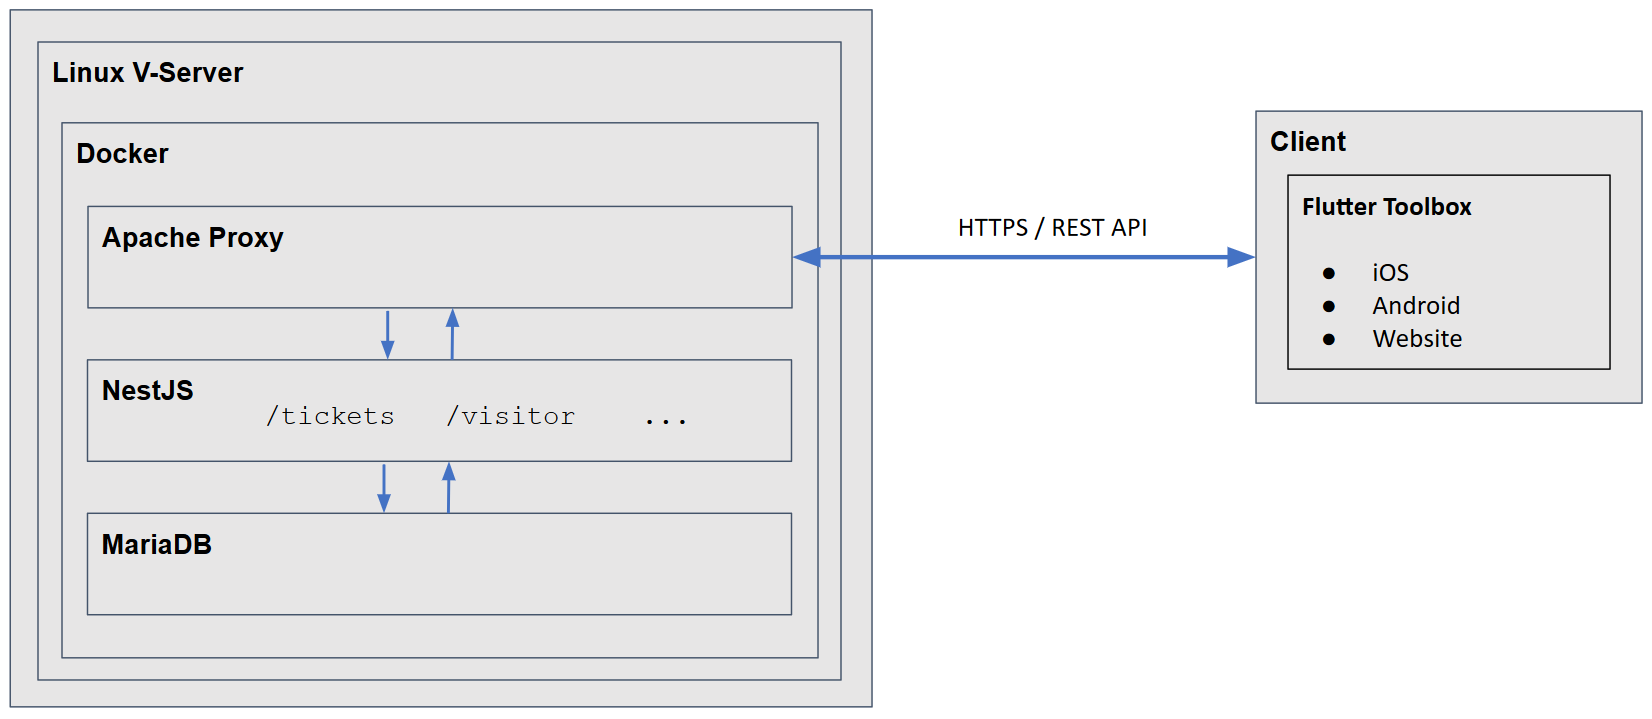
\includegraphics[width=0.9\textwidth]{img/app_architecture.PNG}
    \end{center}
    \caption{Mögliche Architektur einer App für die MOBTS Konferenz}
    \label{fig:architecture}
\end{figure}

\autoref{fig:architecture} zeigt eine Übersicht zu einer möglichen Architektur der App.
Ein Client kommuniziert hier über eine \ac{REST} \ac{API} mit einem Server.
Dabei kann der Client hier sowohl eine Website, als auch eine native Adnroid oder iOS App sein.
Auf dem Server läuft in einem Container ein Proxy, der Anfragen an den Server an die zuständigen Komponenten deligiert.
Der Komponent, der die meisten Anfragen verarbeiten wird, ist eine Node.js Laufzeit Umgebung, auf der ein NestJS Server läuft.
Hier ist die Logik der App implementiert -- Anfragen werden verarbeitet, Daten geladen und gespeichert und Berechtigung überprüft.
Um für Persistenz der Daten zu sorgen läuft in dem Container auch eine Datenbank, in Falle der dargestellten Architektur eine MariaDB, mit der die Node.js Laufzeitumgebung kommuniziert, um Daten zu laden und zu speichern.

\subsection{Technologien}
\subsubsection*{Flutter}
Flutter ist eine von Goolge entwickelte Technologie, die als Werkzeug zur Entwicklung nativer Android und iOS Anwendungen verwendete werden kann.
Dabei müssen Entwickler lediglich einen Code entwickeln, welcher dann von Flutter zu jeweils nativen Android und iOS Applikationen kompiliert wird.
Weiterhin bietet die neuste Version, Flutter 2, erweiterte Möglichkeiten bezüglich der Webeinbindung.
Entwickelte Apps können so einfach auch als Webanwendung bereitgestellt werden.
Damit werden auch nutzer angesprochen, die sich nur für die Konferenz keine App herunterladen wollen. \autocite{B_GoogleDevelopers.} 

\subsubsection*{\ac{REST} \ac{API}}
Eine \ac{API} bezeichnet eine Schnittstelle zwischen Programmen. 
Im Falle der App Entwicklung wird hier primär die Schnittstelle zwischen Back- und Frontend genauerer Betrachtung erfordern.
Grundlegend ist das Backend (der Server) dafür veranwortlich die Logik einer Anwndung, sowie die Datenverarbeitung bereitszustellen.
Diese beinhalten beispielsweise das Anlegen von Nutzerkonten, Authorisierungskonzepte, beispielsweise über Sessions, und das Speichern von Daten.
Das Frontend (die App) ist die Schnittstelle zum Endnutzer, über die mit der Anwendung kommuniziert und interagiert wird.
Dabei ist es Aufgabe der App, Informationen des Servers dem Nutzer anzuzeigen und Eingaben des Nutzers an den Server zu senden. 
Dies geschieht wiederum über die \ac{API}.

\ac{REST} bezeichnet das Architekturprinzip einer API.
Zwar gibt es hier grundlegend keine standardisierte Methoden oder Prinzipien, es können aber einige Kritierien dargelegt werden.
Grundsätzlich setzt eine \ac{REST} \ac{API} eine zustandslose Client/Server-Kommunkation um, was bedeutet, dass es keine gegebene Verbindung zwischen einzelnen Anfragen gibt, wodurch jede Anfrage beispielsweise neu authentifiziert und authorisiert werden muss \autocite{B_RedHat.}.

\begin{figure}[h]
    \begin{center}
        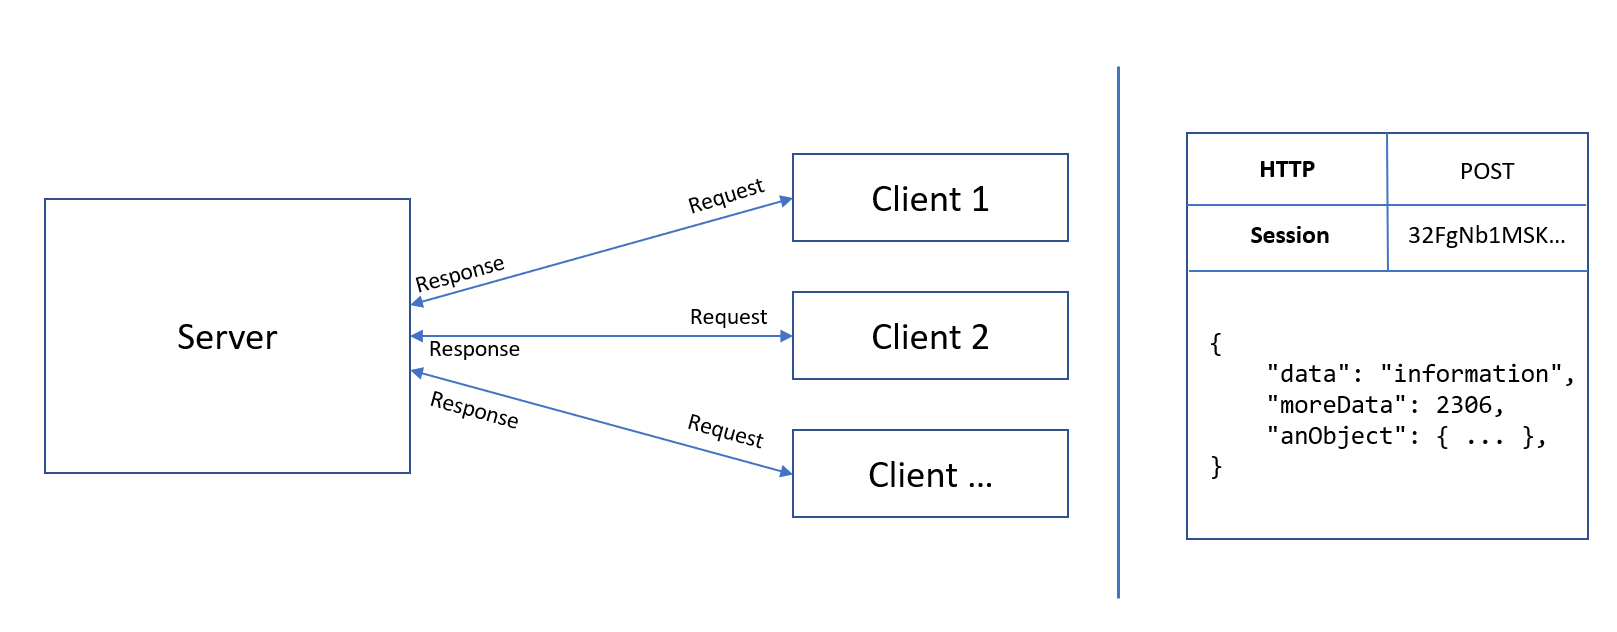
\includegraphics[width=0.9\textwidth]{img/rest_api.PNG}
    \end{center}
    \caption{Grundlegendes Konzept einer REST API}
    \label{fig:rest-api}
\end{figure}

\autoref{fig:rest-api} zeigt vereinfacht das Schema einer \ac{REST} \ac{API}, in der mehrere Clients Anfragen (Request) an einen Server schicken, welche jeweils mit einer Antwort (Response) des Servers beantwortet werden.

\subsubsection*{Docker}
Docker bezeichnet eine beliebte Softwarelösung zur Containerization von Anwendungen.
Containerization bezeichnet dabei das Prinzip Teile einer Anwndung oder eine gesamte Anwendung mit allen Abhängigkeiten, wie externen Code-Bibliotheken in einem Paket einzukapseln.
Ein häufig auftretendes Problem der Software Entwicklung ist, dass Software zwar auf einem System läuft, auf einem anderen aber nicht.
Das ist in sofern problematisch, da Anwender und Unternehmen darauf vertrauen müssen, dass Anwendungen auf allen Systemen gleich laufen.
Um dieses Problem zu lösen, muss entweder ein hoher Aufwand in die Konfiguration von Systemen gesteckt werden, oder das Vertrauen von Anwendern und Unternehmen muss betrogen werden.

Containerization löst dies, indem es das Problem nicht auftreten lässt.
Durch einbindung aller Abhängigkeiten läuft eine Anwendung auf allen Systemen gleich und es bedarf nur eines geringen Konfigurationsaufwands \autocite{B_IBMCloudEducation.2019}.

Docker stellt dabei eine beliebte Lösung der Containerization dar.
Nach einer Umfrage von IBM verwenden bis zu 60\% der Befragten Docker als eine Deployment Platform \autocite{B_IBMCloud.}.
Vorteilhaft an der Verwendung von Mainstream Technologien ist die Existenz einer großen Community und weitereichender Ressourcen zum Anlernen der Technologie.
Auftretende Probleme können auch aufgrund einer größeren Community schnell gelöst werden. 

\subsubsection*{Node.js}
Node.js ist nach eigener Angabe eine asynchrone ereignisgesteuerte JavaScript Laufzeitumgebung. \autocite{Node.js.}
Das bedeutet, dass so wie in einem Webbrowser, in Node.js JavaScript Code ausgeführt werden kann.
Dabei ist Node.js besonders für das Entwickeln von Servern ausgelegt.
Vorteilhaft gegenüber anderer Sprachen ist bei der Entwicklung von JavaScript Servern mit Node.js vor allem die große Community, die sich um Node.js gebildet hat.
Große Communities sind dann immer hilfreich, wenn Probleme auftreten, da entweder Ressourcen im Überfluss zur Verfügung stehen, oder Fragen in Foren schnell von aktiven Vertretern der Community beantwortet werden.
Laut der jährlichen Entwicklerumfrage des Portals Stackoverflow\footnotetext{\url{https://stackoverflow.com/}} verwenden bis zu 50\% aller Befragten Node.js in ihren Projekten -- sowohl privat als auch beruflich \autocite{B_Stackoverflow.2020}.

Weiterhin existieren für Node.js zahlreiche externe Code Bibliotheken, die den Entwicklungsprozess signifikant beschleunigen.
Ebenso gibt es eine große Anzahl an Frameworks, die die Serverentwicklung zu einem gewissen Grad abstrahieren und somit wiederum den Entwicklungsprozess vereinfachen können.
Insbesondere die Auswahl eines passenden Frameworks entscheidet bei der Arbeit mit Node.js über die tatsächliche Umsetzung einer App.

\subsubsection*{NestJS}
NestJS ist ein Node.js basiertes Framework \autocite{B_NestJs.}.
Es ist auf eine Trennung von logisch unabhängigen Programmkomponenten ausgelegt.
Durch diese Entzerrung bleibt eine Anwendung, auch dann wenn sie umfangreicher wird, immernoch übersichtlich.
Grundlegend unterteilt NestJS einen jeweiligen Teil der Geschäftslogik in folgende Komponenten:
\begin{itemize}
    \item \textbf{Controller} sind für das Request/Response Handling verantwortlich, also die Kommunikation mit den Clients.
    \item \textbf{Provider} (Services) sind für die tatsächliche Geschäftslogik veranwortlich. Hier werden die Anfragen der Client verarbeitet und Anworten mit entsprechenden Daten gefüllt.
    \item \textbf{Modules} bieten schließlich die Schnittstelle ziwschen den Komponenten einer NestJS Anwendung.
\end{itemize}
Neben einer übersichtlichen Designphilosophie bietet NestJS weiterhin nativ die Unterstützung der Programmiersprache TypeScript.
TypeScript ist eine Erweiterung der beliebtesten Sprache zur Webentwicklung, JavaScript, welche ebenso beliebt wie auch gefürchtet ist \autocite{B_Stackoverflow.2020}.
Gegenüber JavaScript bietet TypeScript den Vorteil, dass eine statische Typisierung von Valriablen das Entwickeln einfacher macht, da semantische Fehler im Code schneller gefunden und behoben werden können.
Da TypeScript auf JavaScript basiert, ist auch die Lernprozess für Programmierer, die noch nicht mit der Sprache vertraut sind, sehr linear und einfach.
Der Syntax beider Sprachen ist der gleiche, wodurch bereits in JavaScript Gelerntes direkt angewendet werden kann.

\subsubsection*{Datenbank}
Für die praktische Umsetzung einer App für die MOBTS 2022 gilt es in irgendeiner Form Daten zu speichern.
In der Informatik ist die dafür etablierte Lösung in fast jedem Falle eine Datenbank.
Für die meisten Anwendungsfälle etablierte sich in den letzten Jahrzehnten die relationale Datenbank als Standard.
In einer relationalen Datenbank werden Daten nach einem vorher festgelegtem Schema gespeichert \autocite{B_AWS.o.J.}.
Dieses Schema wird im Vorlauf in Form eines ER-Diagramms (Entity Relationship) dargestellt.
Die genaue Struktur eines solchen Diagramms kann erst dann erstellt werden, wenn die praktische Implementierung der App genauer durchdacht wird.
Da diese aber in jedem Fall nicht weit vom \enquote{normalen} Anwendungsfall abweichen wird, sollte eine relationale Datenbank die richtige Wahl sein.
An dieser Stelle sei daher eine relationale, SQL-basierte Datenbank empfohlen, ohne, dass genauer auf deren Strukturierung eingegangen werden soll.
Für die Wahl eines konkreten Datenbankmanagementsystems sei an dieser Stelle MariaDB oder PostgreSQL empfohlen -- beides sind populäre Lösungen, die aus vorher bereits genannten Gründen den Entwicklungsprozess vereinfachen können.